\section*{15.06.2017}



\paragraph{Allgemein}
\begin{itemize}
	\item Einlesen in die Klassen \emph{IGeneralizedRule} (I für Integer) und \emph{GeneralizedRule} um zu 	finden, wie ich die Ersetzungsterme erreichen kann um sie als Lineares Programm aufzufassen
		\begin{figure}[h]
			\centering
			% Graphic for TeX using PGF
% Title: D:\Dokumente\GitHub\Bachelorarbeit\Arbeitstagebuch\src\15.06.2017-classdiagram.dia
% Creator: Dia v0.97.2
% CreationDate: Thu Jun 22 16:42:59 2017
% For: Timo Bergerbusch
% \usepackage{tikz}
% The following commands are not supported in PSTricks at present
% We define them conditionally, so when they are implemented,
% this pgf file will use them.
\ifx\du\undefined
  \newlength{\du}
\fi
\setlength{\du}{15\unitlength}
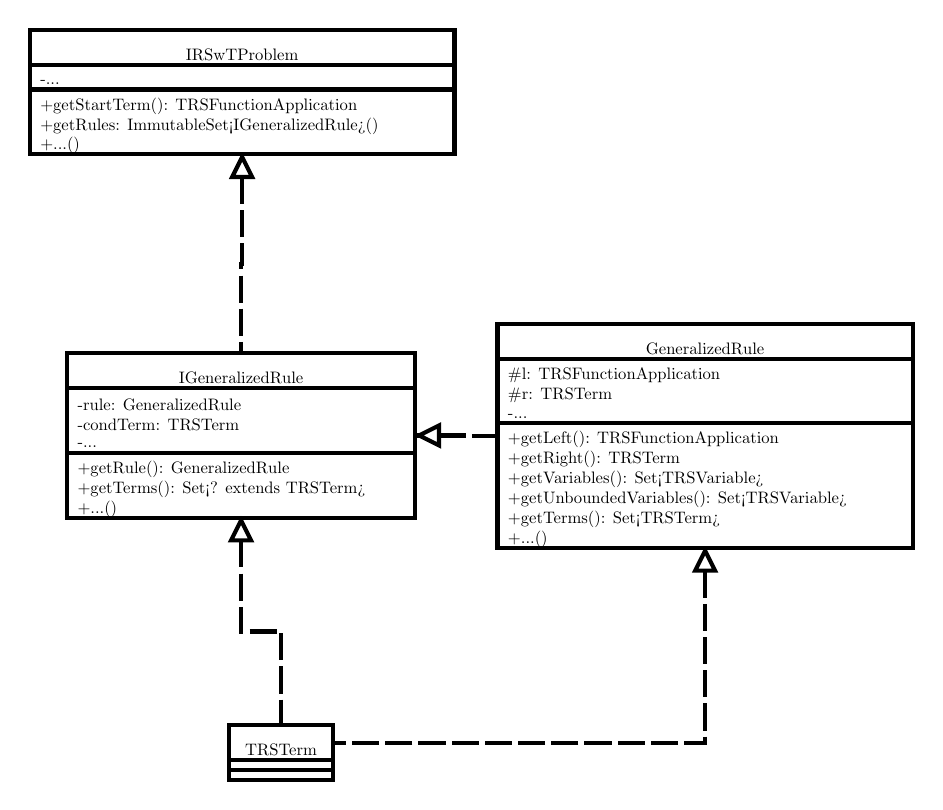
\begin{tikzpicture}[scale=0.6, every node/.style={scale=0.6}]
\pgftransformxscale{1.000000}
\pgftransformyscale{-1.000000}
\definecolor{dialinecolor}{rgb}{0.000000, 0.000000, 0.000000}
\pgfsetstrokecolor{dialinecolor}
\definecolor{dialinecolor}{rgb}{1.000000, 1.000000, 1.000000}
\pgfsetfillcolor{dialinecolor}
\pgfsetlinewidth{0.100000\du}
\pgfsetdash{}{0pt}
\definecolor{dialinecolor}{rgb}{1.000000, 1.000000, 1.000000}
\pgfsetfillcolor{dialinecolor}
\fill (-0.009799\du,0.070962\du)--(-0.009799\du,1.470962\du)--(17.045201\du,1.470962\du)--(17.045201\du,0.070962\du)--cycle;
\definecolor{dialinecolor}{rgb}{0.000000, 0.000000, 0.000000}
\pgfsetstrokecolor{dialinecolor}
\draw (-0.009799\du,0.070962\du)--(-0.009799\du,1.470962\du)--(17.045201\du,1.470962\du)--(17.045201\du,0.070962\du)--cycle;
% setfont left to latex
\definecolor{dialinecolor}{rgb}{0.000000, 0.000000, 0.000000}
\pgfsetstrokecolor{dialinecolor}
\node at (8.517701\du,1.070962\du){IRSwTProblem};
\definecolor{dialinecolor}{rgb}{1.000000, 1.000000, 1.000000}
\pgfsetfillcolor{dialinecolor}
\fill (-0.009799\du,1.470962\du)--(-0.009799\du,2.470962\du)--(17.045201\du,2.470962\du)--(17.045201\du,1.470962\du)--cycle;
\definecolor{dialinecolor}{rgb}{0.000000, 0.000000, 0.000000}
\pgfsetstrokecolor{dialinecolor}
\draw (-0.009799\du,1.470962\du)--(-0.009799\du,2.470962\du)--(17.045201\du,2.470962\du)--(17.045201\du,1.470962\du)--cycle;
% setfont left to latex
\definecolor{dialinecolor}{rgb}{0.000000, 0.000000, 0.000000}
\pgfsetstrokecolor{dialinecolor}
\node[anchor=west] at (0.140201\du,2.130962\du){-...};
\definecolor{dialinecolor}{rgb}{1.000000, 1.000000, 1.000000}
\pgfsetfillcolor{dialinecolor}
\fill (-0.009799\du,2.470962\du)--(-0.009799\du,5.070962\du)--(17.045201\du,5.070962\du)--(17.045201\du,2.470962\du)--cycle;
\definecolor{dialinecolor}{rgb}{0.000000, 0.000000, 0.000000}
\pgfsetstrokecolor{dialinecolor}
\draw (-0.009799\du,2.470962\du)--(-0.009799\du,5.070962\du)--(17.045201\du,5.070962\du)--(17.045201\du,2.470962\du)--cycle;
% setfont left to latex
\definecolor{dialinecolor}{rgb}{0.000000, 0.000000, 0.000000}
\pgfsetstrokecolor{dialinecolor}
\node[anchor=west] at (0.140201\du,3.130962\du){+getStartTerm(): TRSFunctionApplication};
% setfont left to latex
\definecolor{dialinecolor}{rgb}{0.000000, 0.000000, 0.000000}
\pgfsetstrokecolor{dialinecolor}
\node[anchor=west] at (0.140201\du,3.930962\du){+getRules: ImmutableSet<IGeneralizedRule>()};
% setfont left to latex
\definecolor{dialinecolor}{rgb}{0.000000, 0.000000, 0.000000}
\pgfsetstrokecolor{dialinecolor}
\node[anchor=west] at (0.140201\du,4.730962\du){+...()};
\pgfsetlinewidth{0.100000\du}
\pgfsetdash{}{0pt}
\definecolor{dialinecolor}{rgb}{1.000000, 1.000000, 1.000000}
\pgfsetfillcolor{dialinecolor}
\fill (1.486510\du,13.059500\du)--(1.486510\du,14.459500\du)--(15.461510\du,14.459500\du)--(15.461510\du,13.059500\du)--cycle;
\definecolor{dialinecolor}{rgb}{0.000000, 0.000000, 0.000000}
\pgfsetstrokecolor{dialinecolor}
\draw (1.486510\du,13.059500\du)--(1.486510\du,14.459500\du)--(15.461510\du,14.459500\du)--(15.461510\du,13.059500\du)--cycle;
% setfont left to latex
\definecolor{dialinecolor}{rgb}{0.000000, 0.000000, 0.000000}
\pgfsetstrokecolor{dialinecolor}
\node at (8.474010\du,14.059500\du){IGeneralizedRule};
\definecolor{dialinecolor}{rgb}{1.000000, 1.000000, 1.000000}
\pgfsetfillcolor{dialinecolor}
\fill (1.486510\du,14.459500\du)--(1.486510\du,17.059500\du)--(15.461510\du,17.059500\du)--(15.461510\du,14.459500\du)--cycle;
\definecolor{dialinecolor}{rgb}{0.000000, 0.000000, 0.000000}
\pgfsetstrokecolor{dialinecolor}
\draw (1.486510\du,14.459500\du)--(1.486510\du,17.059500\du)--(15.461510\du,17.059500\du)--(15.461510\du,14.459500\du)--cycle;
% setfont left to latex
\definecolor{dialinecolor}{rgb}{0.000000, 0.000000, 0.000000}
\pgfsetstrokecolor{dialinecolor}
\node[anchor=west] at (1.636510\du,15.119500\du){-rule: GeneralizedRule};
% setfont left to latex
\definecolor{dialinecolor}{rgb}{0.000000, 0.000000, 0.000000}
\pgfsetstrokecolor{dialinecolor}
\node[anchor=west] at (1.636510\du,15.919500\du){-condTerm: TRSTerm};
% setfont left to latex
\definecolor{dialinecolor}{rgb}{0.000000, 0.000000, 0.000000}
\pgfsetstrokecolor{dialinecolor}
\node[anchor=west] at (1.636510\du,16.719500\du){-...};
\definecolor{dialinecolor}{rgb}{1.000000, 1.000000, 1.000000}
\pgfsetfillcolor{dialinecolor}
\fill (1.486510\du,17.059500\du)--(1.486510\du,19.659500\du)--(15.461510\du,19.659500\du)--(15.461510\du,17.059500\du)--cycle;
\definecolor{dialinecolor}{rgb}{0.000000, 0.000000, 0.000000}
\pgfsetstrokecolor{dialinecolor}
\draw (1.486510\du,17.059500\du)--(1.486510\du,19.659500\du)--(15.461510\du,19.659500\du)--(15.461510\du,17.059500\du)--cycle;
% setfont left to latex
\definecolor{dialinecolor}{rgb}{0.000000, 0.000000, 0.000000}
\pgfsetstrokecolor{dialinecolor}
\node[anchor=west] at (1.636510\du,17.719500\du){+getRule(): GeneralizedRule};
% setfont left to latex
\definecolor{dialinecolor}{rgb}{0.000000, 0.000000, 0.000000}
\pgfsetstrokecolor{dialinecolor}
\node[anchor=west] at (1.636510\du,18.519500\du){+getTerms(): Set<? extends TRSTerm>};
% setfont left to latex
\definecolor{dialinecolor}{rgb}{0.000000, 0.000000, 0.000000}
\pgfsetstrokecolor{dialinecolor}
\node[anchor=west] at (1.636510\du,19.319500\du){+...()};
\pgfsetlinewidth{0.100000\du}
\pgfsetdash{}{0pt}
\definecolor{dialinecolor}{rgb}{1.000000, 1.000000, 1.000000}
\pgfsetfillcolor{dialinecolor}
\fill (18.769400\du,11.875900\du)--(18.769400\du,13.275900\du)--(35.439400\du,13.275900\du)--(35.439400\du,11.875900\du)--cycle;
\definecolor{dialinecolor}{rgb}{0.000000, 0.000000, 0.000000}
\pgfsetstrokecolor{dialinecolor}
\draw (18.769400\du,11.875900\du)--(18.769400\du,13.275900\du)--(35.439400\du,13.275900\du)--(35.439400\du,11.875900\du)--cycle;
% setfont left to latex
\definecolor{dialinecolor}{rgb}{0.000000, 0.000000, 0.000000}
\pgfsetstrokecolor{dialinecolor}
\node at (27.104400\du,12.875900\du){GeneralizedRule};
\definecolor{dialinecolor}{rgb}{1.000000, 1.000000, 1.000000}
\pgfsetfillcolor{dialinecolor}
\fill (18.769400\du,13.275900\du)--(18.769400\du,15.875900\du)--(35.439400\du,15.875900\du)--(35.439400\du,13.275900\du)--cycle;
\definecolor{dialinecolor}{rgb}{0.000000, 0.000000, 0.000000}
\pgfsetstrokecolor{dialinecolor}
\draw (18.769400\du,13.275900\du)--(18.769400\du,15.875900\du)--(35.439400\du,15.875900\du)--(35.439400\du,13.275900\du)--cycle;
% setfont left to latex
\definecolor{dialinecolor}{rgb}{0.000000, 0.000000, 0.000000}
\pgfsetstrokecolor{dialinecolor}
\node[anchor=west] at (18.919400\du,13.935900\du){\#l: TRSFunctionApplication};
% setfont left to latex
\definecolor{dialinecolor}{rgb}{0.000000, 0.000000, 0.000000}
\pgfsetstrokecolor{dialinecolor}
\node[anchor=west] at (18.919400\du,14.735900\du){\#r: TRSTerm};
% setfont left to latex
\definecolor{dialinecolor}{rgb}{0.000000, 0.000000, 0.000000}
\pgfsetstrokecolor{dialinecolor}
\node[anchor=west] at (18.919400\du,15.535900\du){-...};
\definecolor{dialinecolor}{rgb}{1.000000, 1.000000, 1.000000}
\pgfsetfillcolor{dialinecolor}
\fill (18.769400\du,15.875900\du)--(18.769400\du,20.875900\du)--(35.439400\du,20.875900\du)--(35.439400\du,15.875900\du)--cycle;
\definecolor{dialinecolor}{rgb}{0.000000, 0.000000, 0.000000}
\pgfsetstrokecolor{dialinecolor}
\draw (18.769400\du,15.875900\du)--(18.769400\du,20.875900\du)--(35.439400\du,20.875900\du)--(35.439400\du,15.875900\du)--cycle;
% setfont left to latex
\definecolor{dialinecolor}{rgb}{0.000000, 0.000000, 0.000000}
\pgfsetstrokecolor{dialinecolor}
\node[anchor=west] at (18.919400\du,16.535900\du){+getLeft(): TRSFunctionApplication};
% setfont left to latex
\definecolor{dialinecolor}{rgb}{0.000000, 0.000000, 0.000000}
\pgfsetstrokecolor{dialinecolor}
\node[anchor=west] at (18.919400\du,17.335900\du){+getRight(): TRSTerm};
% setfont left to latex
\definecolor{dialinecolor}{rgb}{0.000000, 0.000000, 0.000000}
\pgfsetstrokecolor{dialinecolor}
\node[anchor=west] at (18.919400\du,18.135900\du){+getVariables(): Set<TRSVariable>};
% setfont left to latex
\definecolor{dialinecolor}{rgb}{0.000000, 0.000000, 0.000000}
\pgfsetstrokecolor{dialinecolor}
\node[anchor=west] at (18.919400\du,18.935900\du){+getUnboundedVariables(): Set<TRSVariable>};
% setfont left to latex
\definecolor{dialinecolor}{rgb}{0.000000, 0.000000, 0.000000}
\pgfsetstrokecolor{dialinecolor}
\node[anchor=west] at (18.919400\du,19.735900\du){+getTerms(): Set<TRSTerm>};
% setfont left to latex
\definecolor{dialinecolor}{rgb}{0.000000, 0.000000, 0.000000}
\pgfsetstrokecolor{dialinecolor}
\node[anchor=west] at (18.919400\du,20.535900\du){+...()};
\pgfsetlinewidth{0.100000\du}
\pgfsetdash{}{0pt}
\definecolor{dialinecolor}{rgb}{1.000000, 1.000000, 1.000000}
\pgfsetfillcolor{dialinecolor}
\fill (8.000000\du,28.000000\du)--(8.000000\du,29.400000\du)--(12.152500\du,29.400000\du)--(12.152500\du,28.000000\du)--cycle;
\definecolor{dialinecolor}{rgb}{0.000000, 0.000000, 0.000000}
\pgfsetstrokecolor{dialinecolor}
\draw (8.000000\du,28.000000\du)--(8.000000\du,29.400000\du)--(12.152500\du,29.400000\du)--(12.152500\du,28.000000\du)--cycle;
% setfont left to latex
\definecolor{dialinecolor}{rgb}{0.000000, 0.000000, 0.000000}
\pgfsetstrokecolor{dialinecolor}
\node at (10.076250\du,29.000000\du){TRSTerm};
\definecolor{dialinecolor}{rgb}{1.000000, 1.000000, 1.000000}
\pgfsetfillcolor{dialinecolor}
\fill (8.000000\du,29.400000\du)--(8.000000\du,29.800000\du)--(12.152500\du,29.800000\du)--(12.152500\du,29.400000\du)--cycle;
\definecolor{dialinecolor}{rgb}{0.000000, 0.000000, 0.000000}
\pgfsetstrokecolor{dialinecolor}
\draw (8.000000\du,29.400000\du)--(8.000000\du,29.800000\du)--(12.152500\du,29.800000\du)--(12.152500\du,29.400000\du)--cycle;
\definecolor{dialinecolor}{rgb}{1.000000, 1.000000, 1.000000}
\pgfsetfillcolor{dialinecolor}
\fill (8.000000\du,29.800000\du)--(8.000000\du,30.200000\du)--(12.152500\du,30.200000\du)--(12.152500\du,29.800000\du)--cycle;
\definecolor{dialinecolor}{rgb}{0.000000, 0.000000, 0.000000}
\pgfsetstrokecolor{dialinecolor}
\draw (8.000000\du,29.800000\du)--(8.000000\du,30.200000\du)--(12.152500\du,30.200000\du)--(12.152500\du,29.800000\du)--cycle;
\pgfsetlinewidth{0.100000\du}
\pgfsetdash{{1.000000\du}{1.000000\du}}{0\du}
\pgfsetdash{{0.400000\du}{0.400000\du}}{0\du}
\pgfsetmiterjoin
\pgfsetbuttcap
{
\definecolor{dialinecolor}{rgb}{0.000000, 0.000000, 0.000000}
\pgfsetfillcolor{dialinecolor}
% was here!!!
\definecolor{dialinecolor}{rgb}{0.000000, 0.000000, 0.000000}
\pgfsetstrokecolor{dialinecolor}
\draw (8.517701\du,5.070962\du)--(8.517701\du,9.465231\du)--(8.474010\du,9.465231\du)--(8.474010\du,13.059500\du);
}
\definecolor{dialinecolor}{rgb}{0.000000, 0.000000, 0.000000}
\pgfsetstrokecolor{dialinecolor}
\draw (8.517701\du,5.982766\du)--(8.517701\du,9.465231\du)--(8.474010\du,9.465231\du)--(8.474010\du,13.059500\du);
\pgfsetmiterjoin
\definecolor{dialinecolor}{rgb}{1.000000, 1.000000, 1.000000}
\pgfsetfillcolor{dialinecolor}
\fill (8.917701\du,5.982766\du)--(8.517701\du,5.182766\du)--(8.117701\du,5.982766\du)--cycle;
\pgfsetlinewidth{0.100000\du}
\pgfsetdash{}{0pt}
\pgfsetmiterjoin
\definecolor{dialinecolor}{rgb}{0.000000, 0.000000, 0.000000}
\pgfsetstrokecolor{dialinecolor}
\draw (8.917701\du,5.982766\du)--(8.517701\du,5.182766\du)--(8.117701\du,5.982766\du)--cycle;
% setfont left to latex
\pgfsetlinewidth{0.100000\du}
\pgfsetdash{{0.400000\du}{0.400000\du}}{0\du}
\pgfsetdash{{0.400000\du}{0.400000\du}}{0\du}
\pgfsetmiterjoin
\pgfsetbuttcap
{
\definecolor{dialinecolor}{rgb}{0.000000, 0.000000, 0.000000}
\pgfsetfillcolor{dialinecolor}
% was here!!!
\definecolor{dialinecolor}{rgb}{0.000000, 0.000000, 0.000000}
\pgfsetstrokecolor{dialinecolor}
\draw (15.511940\du,16.359500\du)--(17.540670\du,16.359500\du)--(17.540670\du,16.375900\du)--(18.769400\du,16.375900\du);
}
\definecolor{dialinecolor}{rgb}{0.000000, 0.000000, 0.000000}
\pgfsetstrokecolor{dialinecolor}
\draw (16.423743\du,16.359500\du)--(17.540670\du,16.359500\du)--(17.540670\du,16.375900\du)--(18.769400\du,16.375900\du);
\pgfsetmiterjoin
\definecolor{dialinecolor}{rgb}{1.000000, 1.000000, 1.000000}
\pgfsetfillcolor{dialinecolor}
\fill (16.423743\du,15.959500\du)--(15.623743\du,16.359500\du)--(16.423743\du,16.759500\du)--cycle;
\pgfsetlinewidth{0.100000\du}
\pgfsetdash{}{0pt}
\pgfsetmiterjoin
\definecolor{dialinecolor}{rgb}{0.000000, 0.000000, 0.000000}
\pgfsetstrokecolor{dialinecolor}
\draw (16.423743\du,15.959500\du)--(15.623743\du,16.359500\du)--(16.423743\du,16.759500\du)--cycle;
% setfont left to latex
\pgfsetlinewidth{0.100000\du}
\pgfsetdash{{0.400000\du}{0.400000\du}}{0\du}
\pgfsetdash{{0.400000\du}{0.400000\du}}{0\du}
\pgfsetmiterjoin
\pgfsetbuttcap
{
\definecolor{dialinecolor}{rgb}{0.000000, 0.000000, 0.000000}
\pgfsetfillcolor{dialinecolor}
% was here!!!
\definecolor{dialinecolor}{rgb}{0.000000, 0.000000, 0.000000}
\pgfsetstrokecolor{dialinecolor}
\draw (8.474010\du,19.659500\du)--(8.474010\du,24.229750\du)--(10.076250\du,24.229750\du)--(10.076250\du,28.000000\du);
}
\definecolor{dialinecolor}{rgb}{0.000000, 0.000000, 0.000000}
\pgfsetstrokecolor{dialinecolor}
\draw (8.474010\du,20.571303\du)--(8.474010\du,24.229750\du)--(10.076250\du,24.229750\du)--(10.076250\du,28.000000\du);
\pgfsetmiterjoin
\definecolor{dialinecolor}{rgb}{1.000000, 1.000000, 1.000000}
\pgfsetfillcolor{dialinecolor}
\fill (8.874010\du,20.571303\du)--(8.474010\du,19.771303\du)--(8.074010\du,20.571303\du)--cycle;
\pgfsetlinewidth{0.100000\du}
\pgfsetdash{}{0pt}
\pgfsetmiterjoin
\definecolor{dialinecolor}{rgb}{0.000000, 0.000000, 0.000000}
\pgfsetstrokecolor{dialinecolor}
\draw (8.874010\du,20.571303\du)--(8.474010\du,19.771303\du)--(8.074010\du,20.571303\du)--cycle;
% setfont left to latex
\pgfsetlinewidth{0.100000\du}
\pgfsetdash{{0.400000\du}{0.400000\du}}{0\du}
\pgfsetdash{{0.400000\du}{0.400000\du}}{0\du}
\pgfsetmiterjoin
\pgfsetbuttcap
{
\definecolor{dialinecolor}{rgb}{0.000000, 0.000000, 0.000000}
\pgfsetfillcolor{dialinecolor}
% was here!!!
\definecolor{dialinecolor}{rgb}{0.000000, 0.000000, 0.000000}
\pgfsetstrokecolor{dialinecolor}
\draw (27.104400\du,20.875900\du)--(27.104400\du,28.700000\du)--(12.152500\du,28.700000\du);
}
\definecolor{dialinecolor}{rgb}{0.000000, 0.000000, 0.000000}
\pgfsetstrokecolor{dialinecolor}
\draw (27.104400\du,21.787703\du)--(27.104400\du,28.700000\du)--(12.152500\du,28.700000\du);
\pgfsetmiterjoin
\definecolor{dialinecolor}{rgb}{1.000000, 1.000000, 1.000000}
\pgfsetfillcolor{dialinecolor}
\fill (27.504400\du,21.787703\du)--(27.104400\du,20.987703\du)--(26.704400\du,21.787703\du)--cycle;
\pgfsetlinewidth{0.100000\du}
\pgfsetdash{}{0pt}
\pgfsetmiterjoin
\definecolor{dialinecolor}{rgb}{0.000000, 0.000000, 0.000000}
\pgfsetstrokecolor{dialinecolor}
\draw (27.504400\du,21.787703\du)--(27.104400\du,20.987703\du)--(26.704400\du,21.787703\du)--cycle;
% setfont left to latex
\end{tikzpicture}

			\caption{Das Klassendiagram des IRSwTProblem und seinen Komponenten zum besseren Verständnis der notwendigen Programmteile. Stand: 15.06.2017}
			\label{15.06.2017:: IRSwTProblem-classdiagram}
		\end{figure}
\end{itemize}
